% Created 2020-06-08 Mon 10:49
% Intended LaTeX compiler: pdflatex
\documentclass[presentation]{beamer}
\usepackage[utf8]{inputenc}
\usepackage[T1]{fontenc}
\usepackage{graphicx}
\usepackage{grffile}
\usepackage{longtable}
\usepackage{wrapfig}
\usepackage{rotating}
\usepackage[normalem]{ulem}
\usepackage{amsmath}
\usepackage{textcomp}
\usepackage{amssymb}
\usepackage{capt-of}
\usepackage{hyperref}
\usetheme{UoB}
\author{Mark Blyth}
\date{\textit{[2020-06-08 Mon]}}
\title{\emph{(More)} surrogate modelling}
\hypersetup{
 pdfauthor={Mark Blyth},
 pdftitle={\emph{(More)} surrogate modelling},
 pdfkeywords={},
 pdfsubject={},
 pdfcreator={Emacs 26.3 (Org mode 9.1.9)}, 
 pdflang={English}}
\begin{document}

\maketitle

\section{Background}
\label{sec:org3a4ab46}
\begin{frame}[label={sec:org5842576}]{Week's goal}
Keep working through different regression models:
\vfill
\begin{itemize}
\item \alert{Function-space distribution over kernels}
\item \alert{Matern kernels}
\item \alert{Bayesian free-knot splines}
\item \sout{Generalised spectral mixture kernels}
\item Switching kernel
\item NARMAX
\item Neural ODEs
\end{itemize}
\end{frame}

\begin{frame}[label={sec:orga71ed93}]{Week's goal}
\begin{itemize}
\item \alert{Function-space distribution over kernels}
\begin{itemize}
\item Works, but no better than the other stationary kernels \emph{[why not?]}
\end{itemize}
\item \alert{Matern kernels}
\begin{itemize}
\item Works, but doesn't average noise out \emph{[lengthscale issue]}
\end{itemize}
\item \alert{Bayesian free-knot splines}
\begin{itemize}
\item Works well!
\end{itemize}
\item \sout{Generalised spectral mixture kernels}
\begin{itemize}
\item Couldn't get them to train
\end{itemize}
\end{itemize}
\end{frame}


\section{Matern kernel}
\label{sec:orgfcf16e8}
\begin{frame}[label={sec:org317d848}]{Matern kernel}
\begin{itemize}
\item SEKernel is \(C^\infty\) smooth
\item Matern kernel generalises this to arbitrary degrees of smoothness
\item Matern \(\frac{3}{2}\) and \(\frac{5}{2}\) are most commonly used
\begin{itemize}
\item Once- and twice- differentiable posteriors
\end{itemize}
\item Lack of smoothness adds more flexibility
\item Quick and easy to test!
\end{itemize}
\end{frame}

\begin{frame}[plain,label={sec:orgce8e801}]{Can sometimes smooth data}
\begin{columns}
\begin{column}{0.5\columnwidth}
\begin{center}
Hindmarsh-Rose fast
\end{center}

\begin{center}
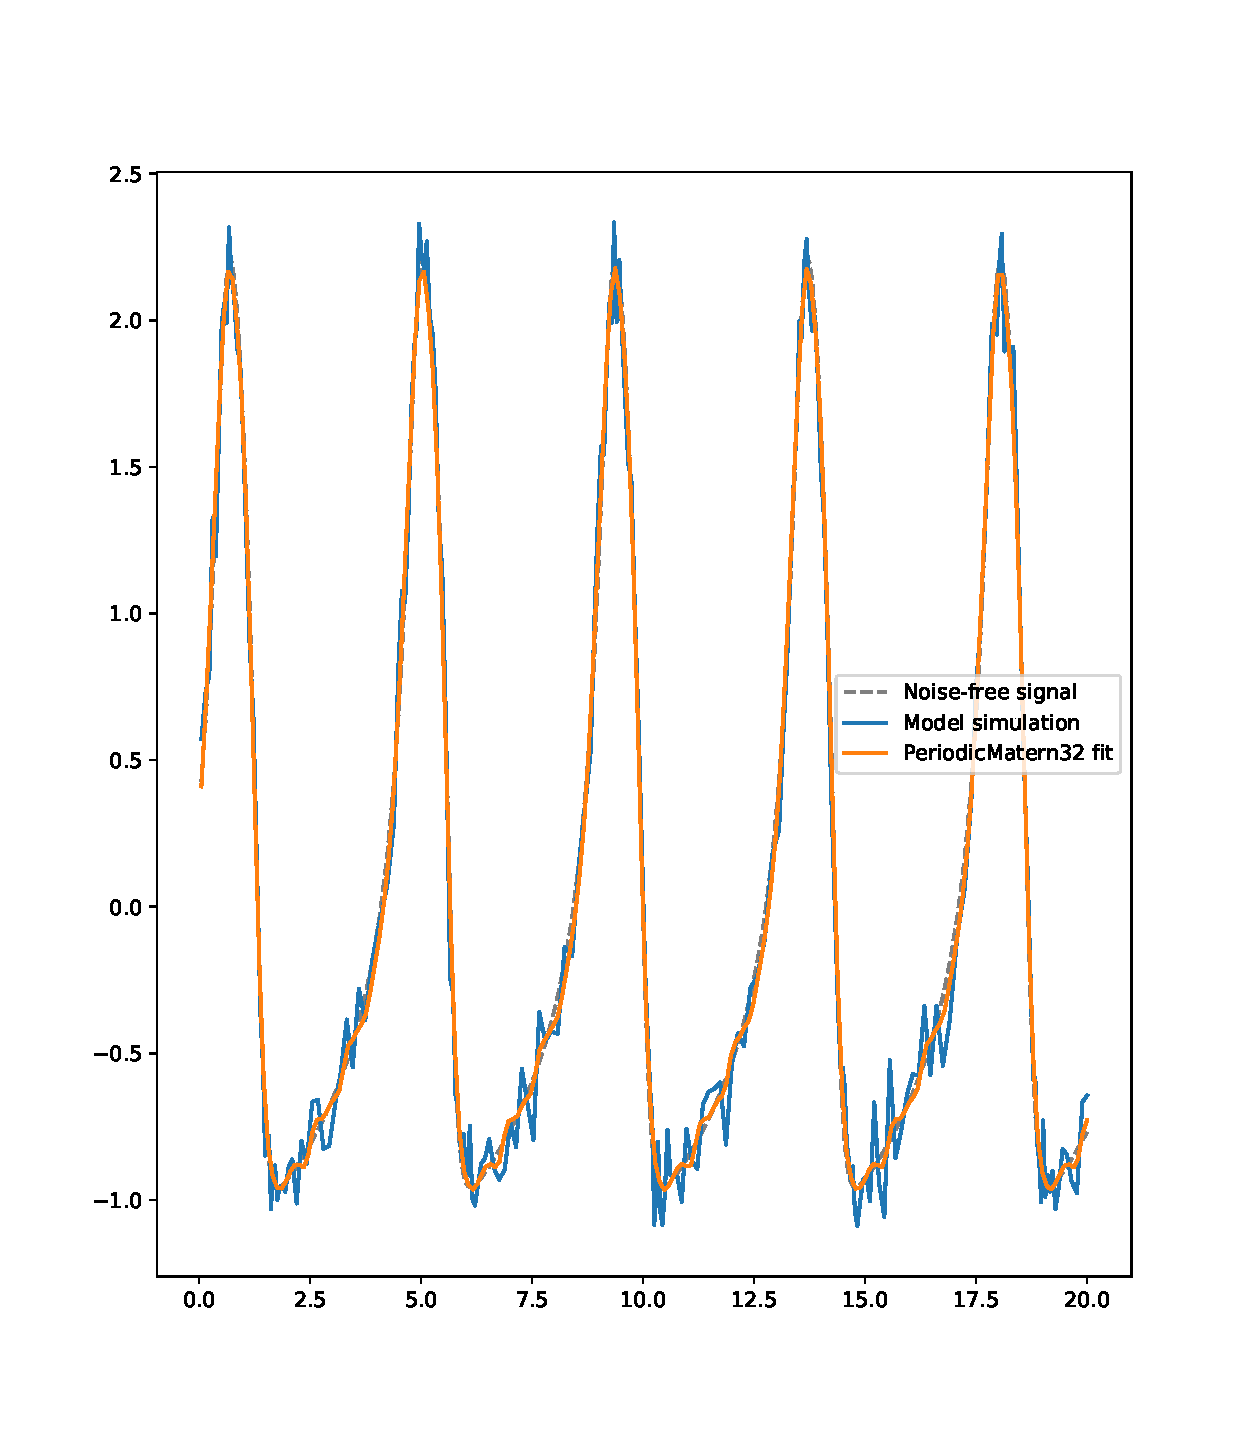
\includegraphics[width=1.1\textwidth]{./Matern1.pdf}
\end{center}
\end{column}

\begin{column}{0.5\columnwidth}
\begin{center}
Hindmarsh-Rose fast
\end{center}

\begin{center}
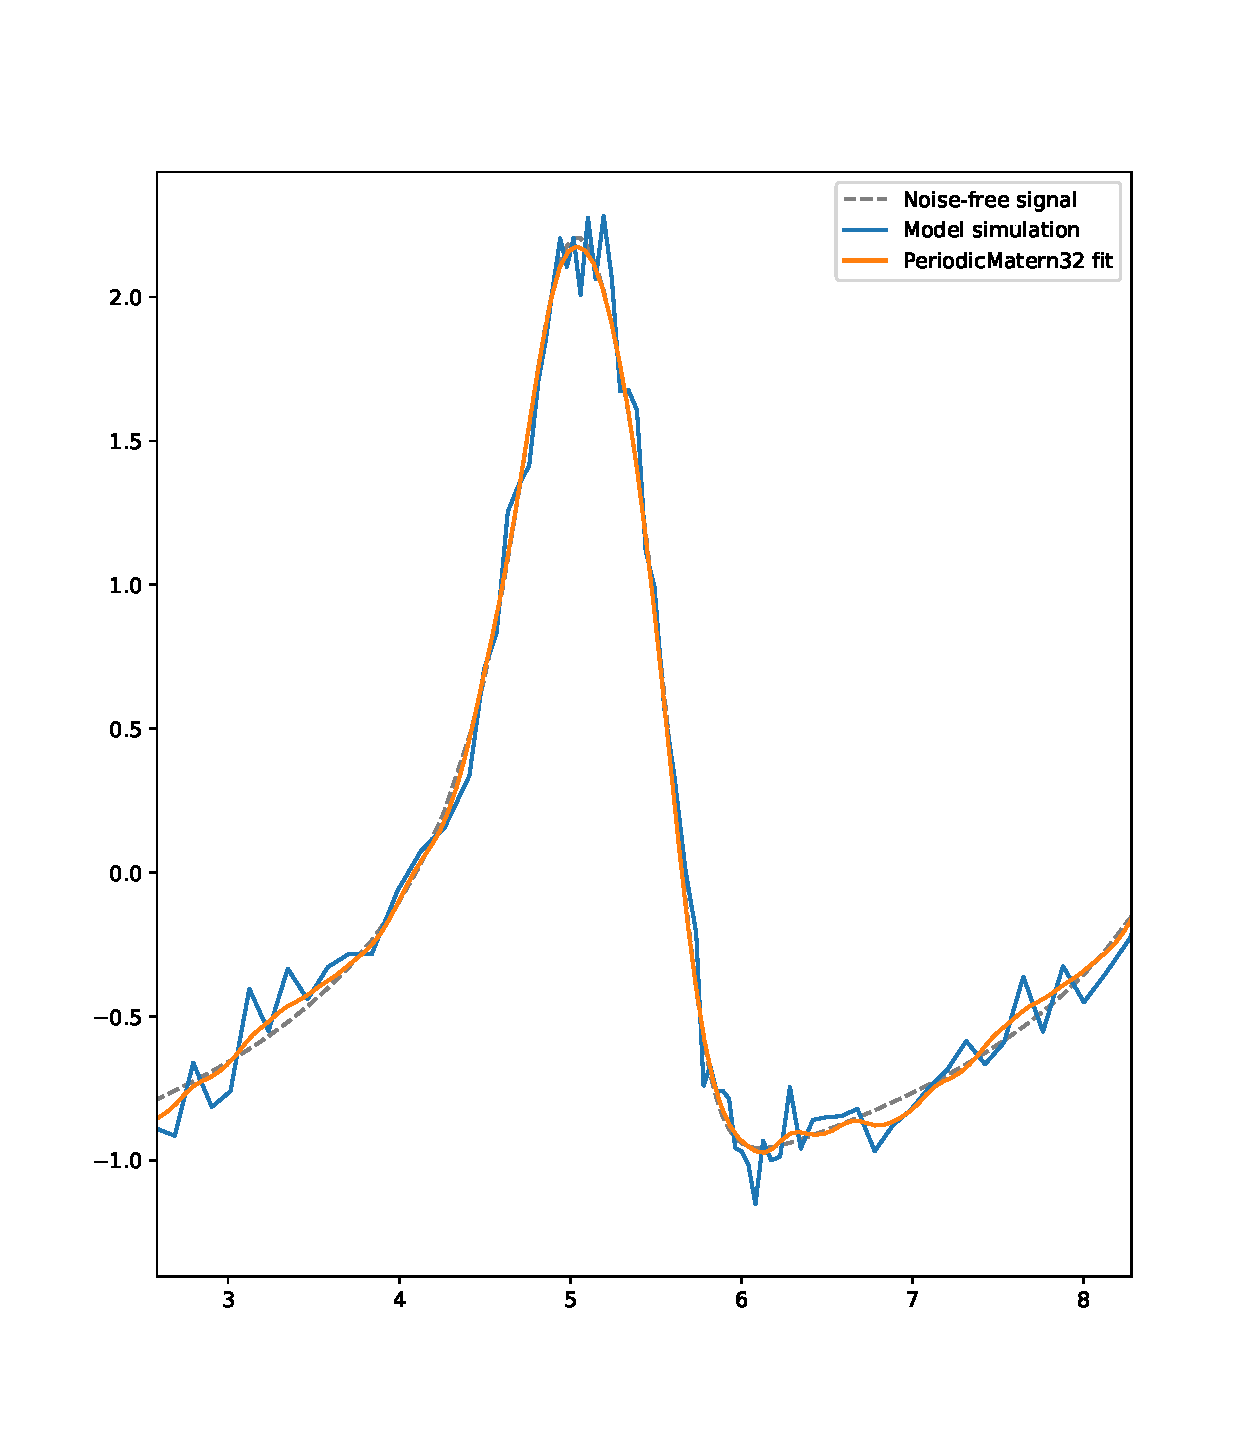
\includegraphics[width=1.1\textwidth]{./Matern2.pdf}
\end{center}
\end{column}
\end{columns}
\end{frame}

\begin{frame}[plain,label={sec:org0c224a2}]{\ldots{}but not always}
\begin{columns}
\begin{column}{0.5\columnwidth}
\begin{center}
Hodgkin-Huxley
\end{center}

\begin{center}
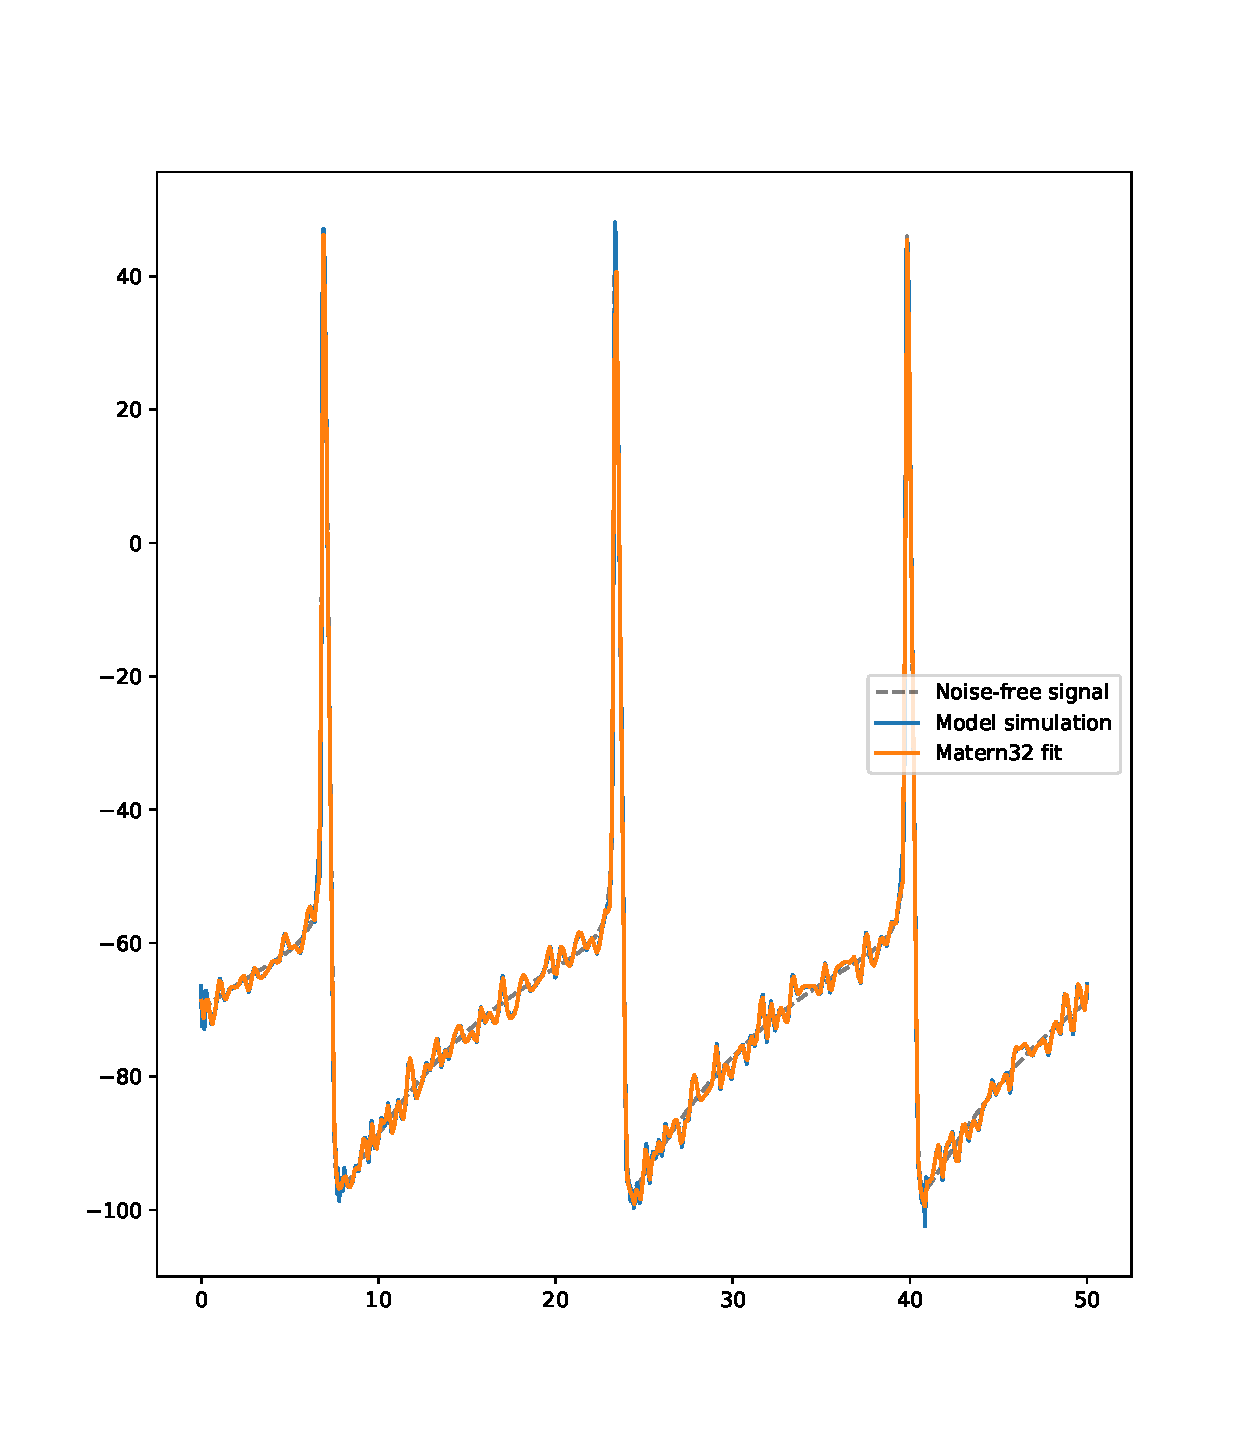
\includegraphics[width=1.1\textwidth]{./Matern4.pdf}
\end{center}
\end{column}

\begin{column}{0.5\columnwidth}
\begin{center}
Hodgkin-Huxley
\end{center}

\begin{center}
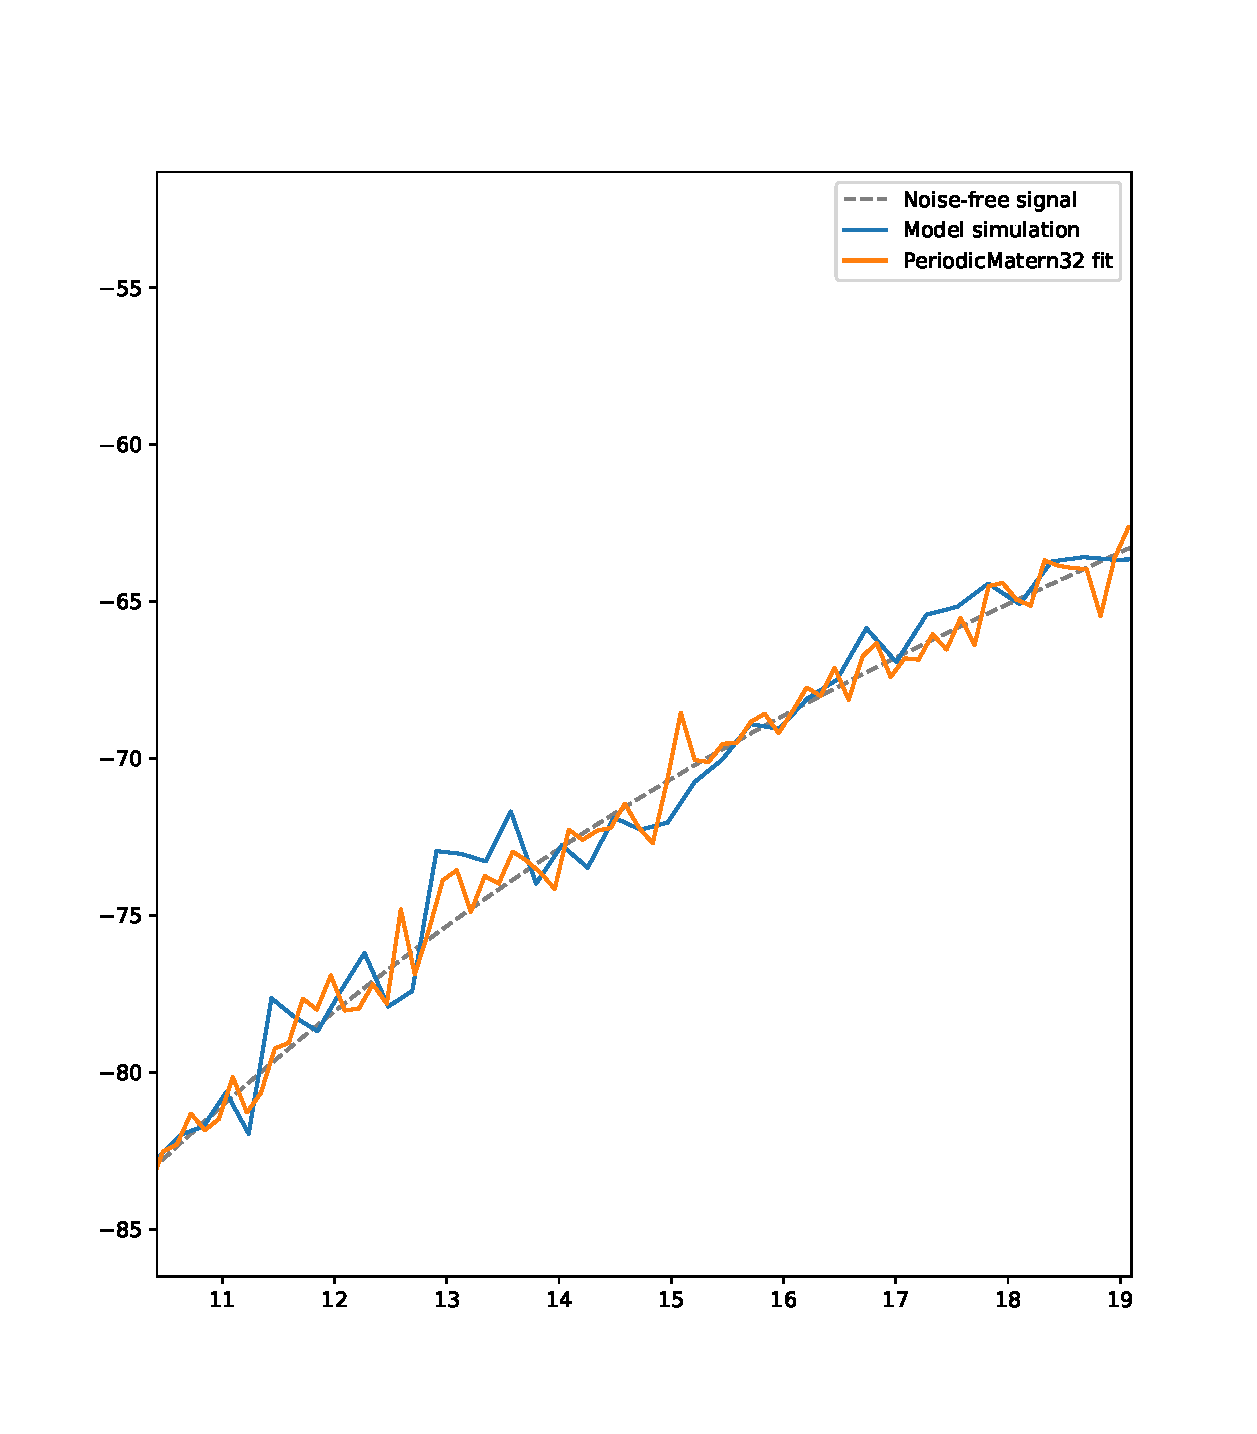
\includegraphics[width=1.1\textwidth]{./Matern3.pdf}
\end{center}
\end{column}
\end{columns}
\end{frame}

\begin{frame}[plain,label={sec:orgc853557}]{\ldots{}but not always}
\begin{columns}
\begin{column}{0.5\columnwidth}
\begin{center}
Real data
\end{center}

\begin{center}
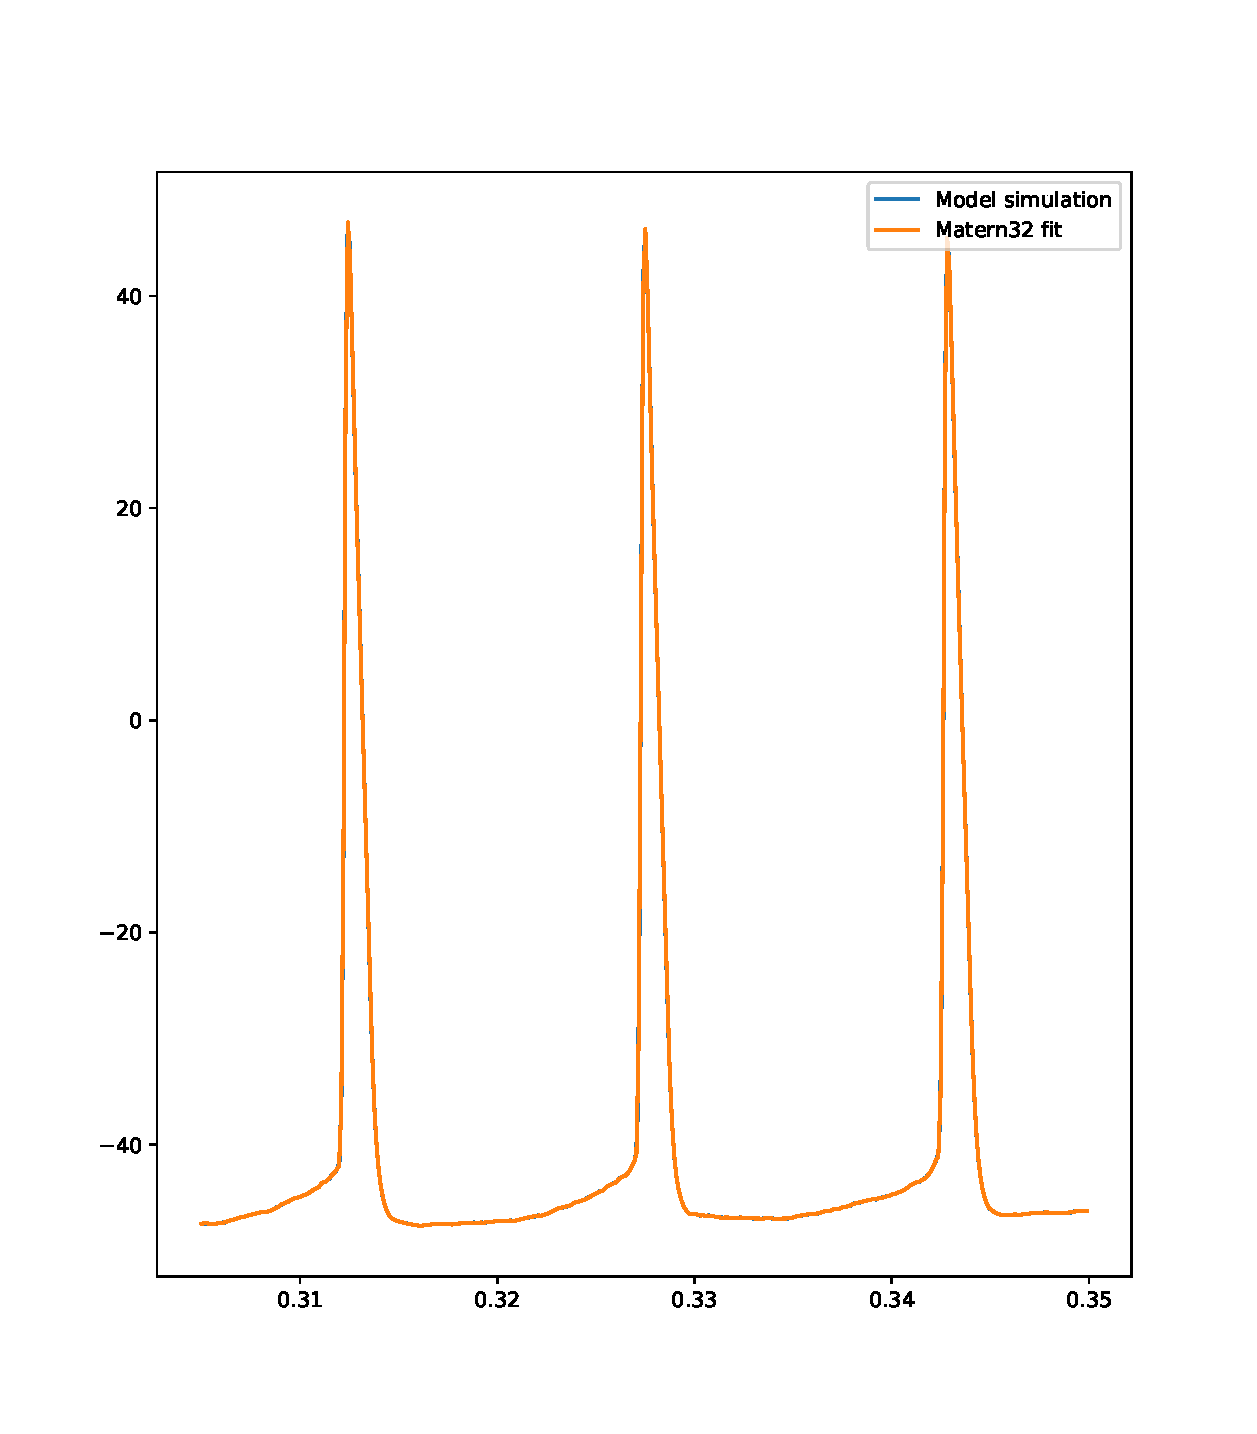
\includegraphics[width=1.1\textwidth]{./Matern5.pdf}
\end{center}
\end{column}

\begin{column}{0.5\columnwidth}
\begin{center}
Real data
\end{center}

\begin{center}
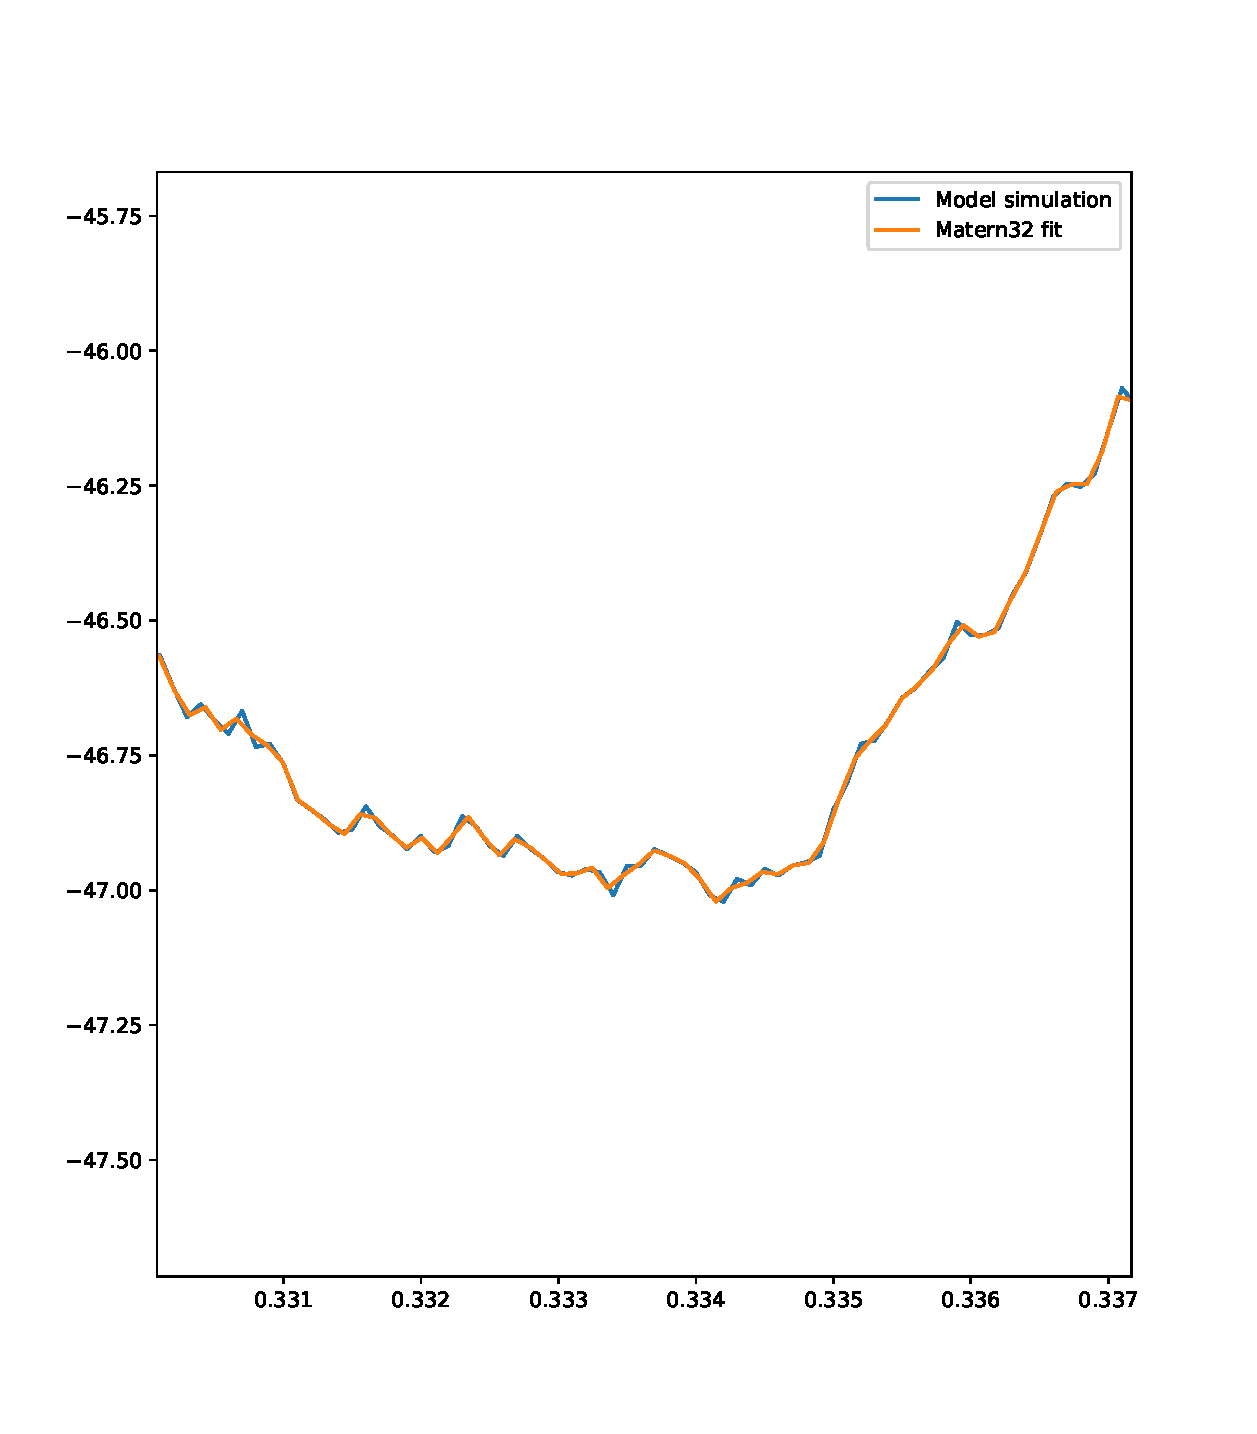
\includegraphics[width=1.1\textwidth]{./Matern6.pdf}
\end{center}
\end{column}
\end{columns}
\end{frame}


\section{MSPEs}
\label{sec:orgc0a7457}
\begin{frame}[label={sec:orgc27909d}]{MSPEs}
Exactly how good are any fits?
\vfill
\begin{itemize}
\item Mean-square prediction error can quantify the goodness-of-fit with synthetic data
\begin{itemize}
\item Split synthetic data into test and training
\item Fit model on training data
\item Find prediction error from test data
\end{itemize}
\end{itemize}

\vfill

The downsampling step causes problems with a GPR fit
\end{frame}

\begin{frame}[plain,label={sec:org23978bc}]{Model fits}
\begin{columns}
\begin{column}{0.5\columnwidth}
\begin{center}
Downsampled 666 to 333 datapoints
\end{center}
\begin{center}
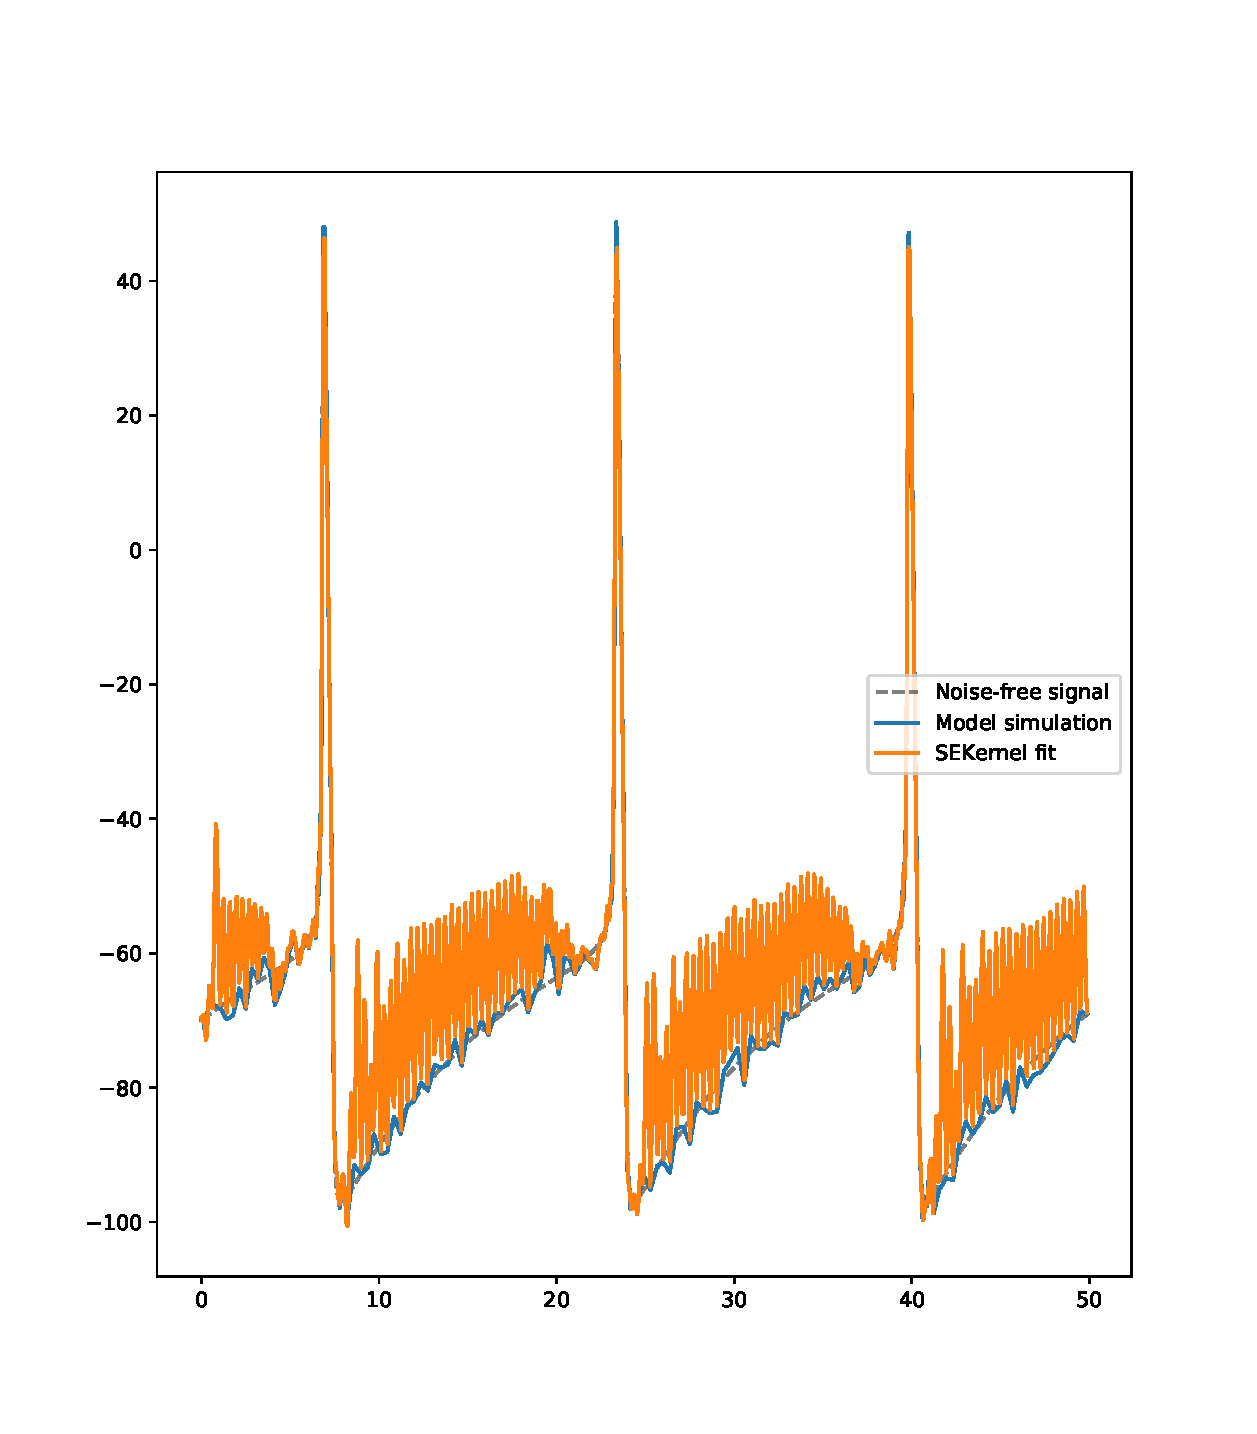
\includegraphics[width=1.1\textwidth]{./downsample333.pdf}
\end{center}
\end{column}

\begin{column}{0.5\columnwidth}
\begin{center}
Simulated with 348 datapoints
\end{center}
\begin{center}
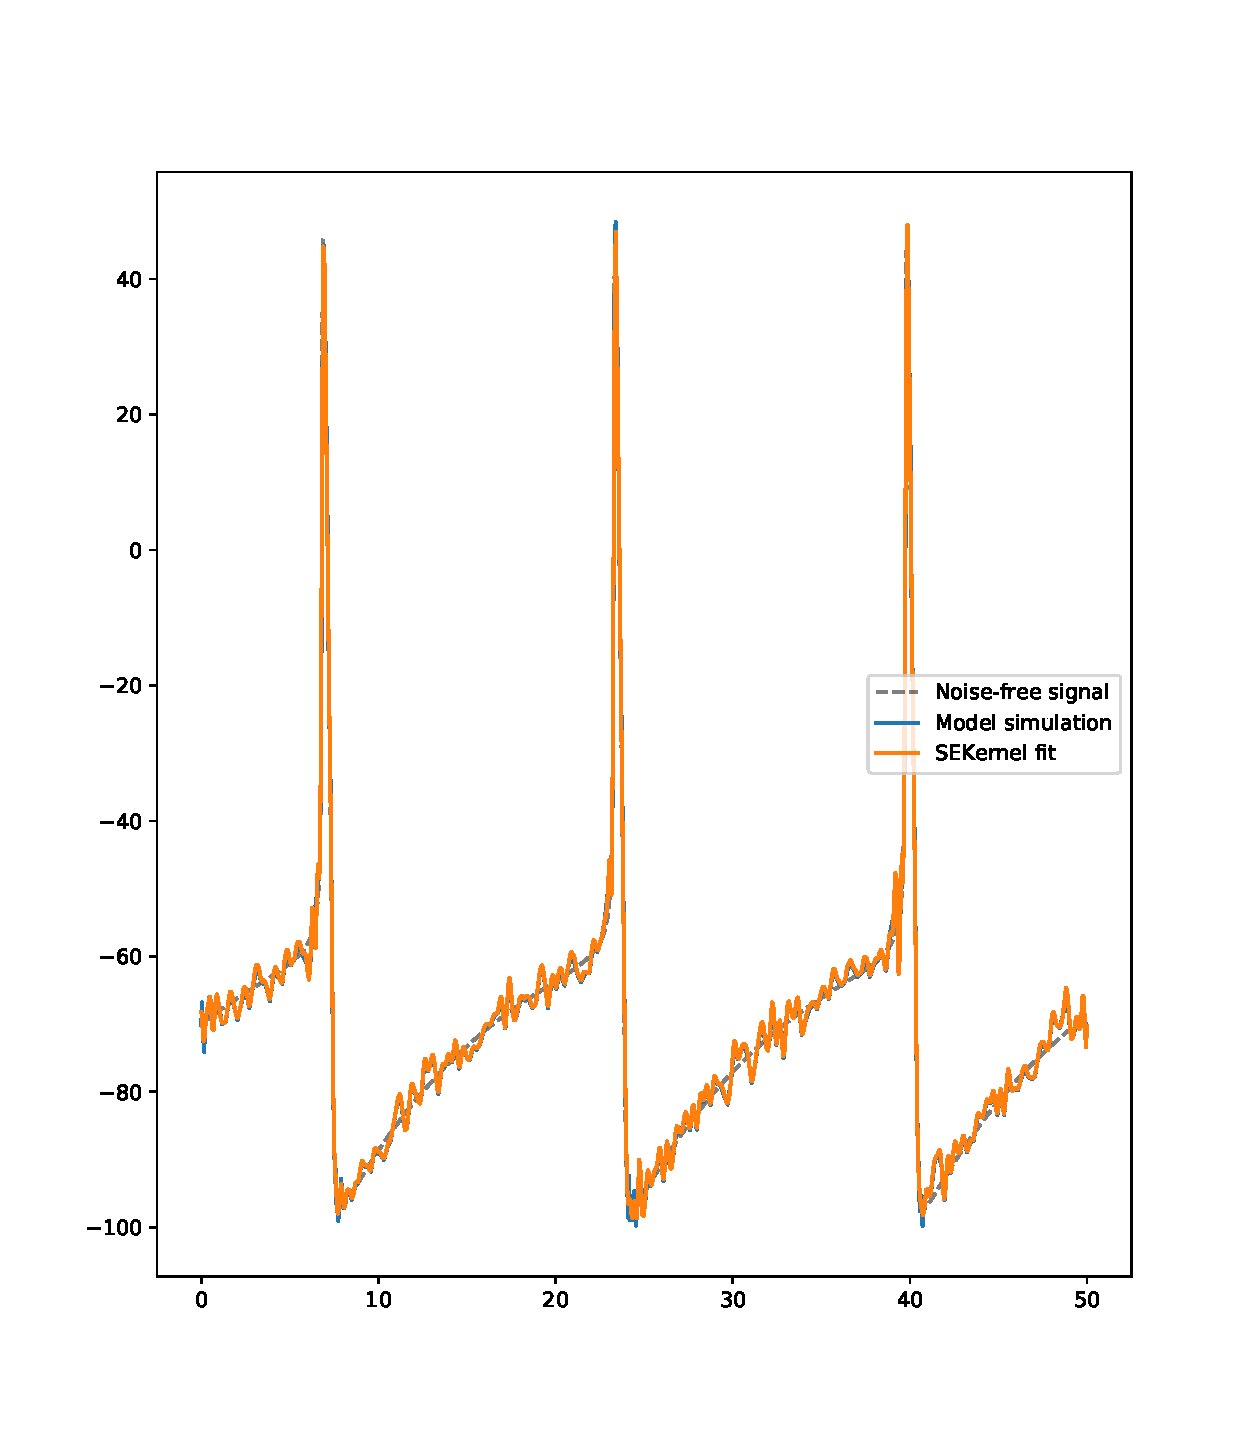
\includegraphics[width=1.1\textwidth]{./nodownsample.pdf}
\end{center}
\end{column}
\end{columns}
\end{frame}

\begin{frame}[label={sec:orgcfd6836}]{MSPEs}
Validation results can't always be trusted - MSPE values are often too high.
Possible hand-wavy explanation:
\begin{itemize}[<+->]
\item More datapoints were generated by tightning the ODE solver tolerance
\item ODE solvers use an adaptive stepsize
\begin{itemize}
\item More datapoints where the system is locally stiff
\item Datapoints are therefore chosen to be as informative as possible
\item Placed at points with the largest margin for error, to zero this error
\end{itemize}
\item Changing \emph{rtol} always gives a maximally informative dataset, for the number of points
\item Downsampling doesn't always give maximally informative data
\begin{itemize}
\item Removes datapoints based on their indices, rather than informativeness
\end{itemize}
\item Less informative dataset means worse GPR fit
\end{itemize}
\end{frame}

\begin{frame}[label={sec:orgb680401}]{Fixing MSPE}
Alternative approaches to MSPE:
\begin{itemize}
\item Leave-one-out cross validation 
\begin{itemize}
\item Computationally expensive
\end{itemize}
\item Visual inspection
\begin{itemize}
\item Subjective, imprecise
\end{itemize}
\item Run two solvers, one for test and one for training data
\begin{itemize}
\item Need to make sure there's no shared datapoints for this to work
\item Bad test if test and training points are very close to each other
\end{itemize}
\end{itemize}
\vfill
MSPE only seems to break on PeriodicKernels or Hodgkin Huxley dataset
\begin{itemize}
\item Chosen approach: use MSPE as-is, but do it carefully
\end{itemize}
\end{frame}

\begin{frame}[label={sec:org6710978}]{Real data}
\begin{itemize}
\item Real data is the best test of a regression model
\item Lack of ground-truth makes it harder to evaluate models on real data
\item A heuristic method:
\begin{itemize}
\item Fit model
\item Look at the model fit
\item Find residuals
\item Look at their distribution
\end{itemize}
\end{itemize}
\end{frame}

\begin{frame}[label={sec:org48a5efc}]{Real data, splines model}
\begin{center}
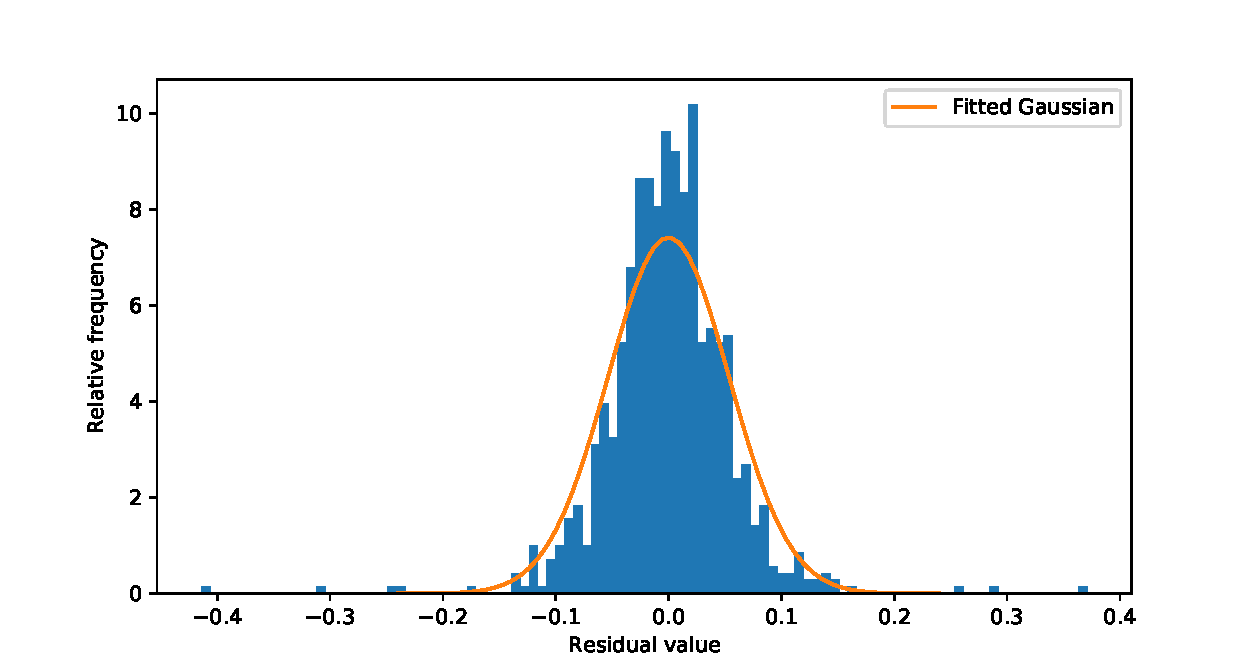
\includegraphics[width=.9\textwidth]{./hist.pdf}
\end{center}
\vfill
\end{frame}

\begin{frame}[label={sec:org5f5781c}]{Real data}
\begin{columns}
\begin{column}{0.5\columnwidth}
\begin{center}
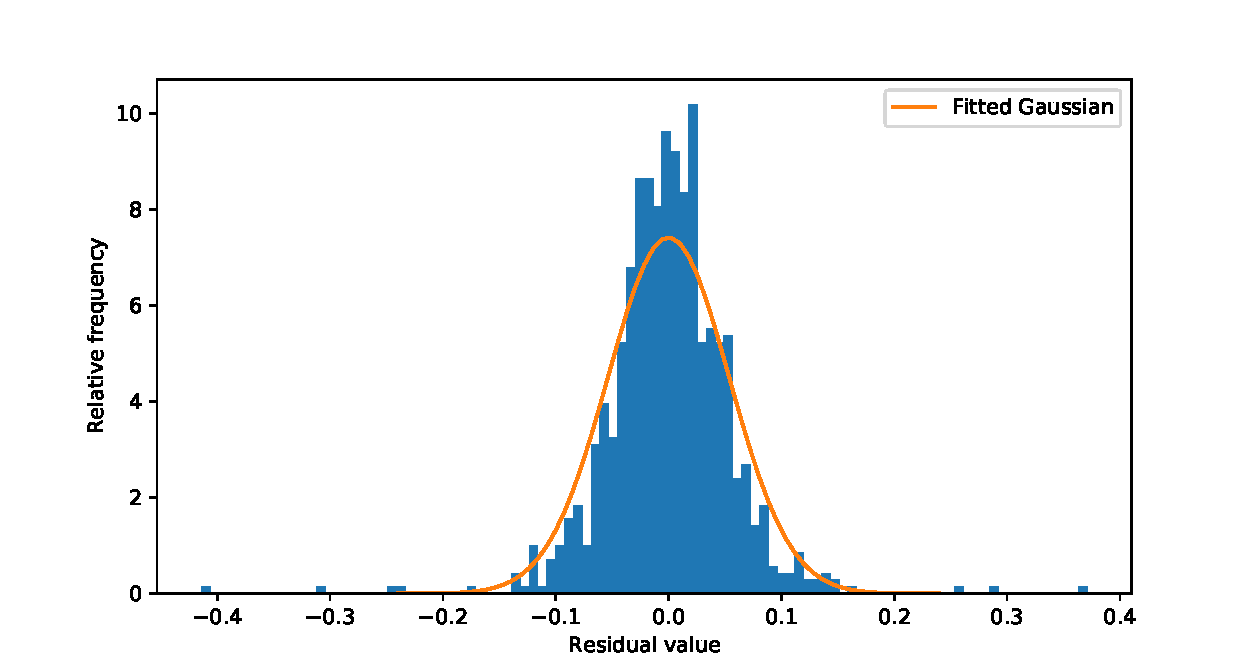
\includegraphics[width=\textwidth]{./hist.pdf}
\end{center}
\end{column}

\begin{column}{0.5\columnwidth}
\begin{itemize}
\item Nothing particularly alarming about the residuals
\begin{itemize}
\item That's all we can really say
\end{itemize}
\item \sout{H\(_{\text{0}}\): residuals are Gaussian} \emph{\alert{[rejected]}}
\begin{itemize}
\item Shapiro-Wilk p-value: 3.0734860972720244e-21
\item D'Agostino's K\(^{\text{2}}\) test: 4.3027710773715154e-37
\end{itemize}
\end{itemize}
\end{column}
\end{columns}
\end{frame}

\begin{frame}[label={sec:org02a4e79}]{Calculated MSPEs}
\begin{center}
\begin{tabular}{lrlrr}
\hline
Model & Matern32 & Matern52 & SEKernel & PeriodicKernel\\
\hline
Hodgkin Huxley & \alert{2.26(-2)} & 2.67\,(-1) & 5.57 & 9.25\\
Fitzhugh Nagumo & 5.37\,(-7) & \alert{2.34(-8)} & 2.97\,(-4) & 2.21\,(-2)\\
HRFast & 1.48\,(-7) & \alert{4.30(-9)} & 2.37\,(-6) & 1.22\,(-2)\\
\hline
\end{tabular}
\end{center}

\begin{itemize}
\item Calculated on noise-free models
\item Matern kernels perform the best
\item Can't compare MSPEs across neuron models, since it scales with the square of signal amplitude
\end{itemize}
\end{frame}

\begin{frame}[label={sec:orga15dd39}]{Calculated MSPEs}
\begin{center}
\begin{tabular}{lrrrr}
\hline
Model & Matern32 & Matern52 & SEKernel & PeriodicKernel\\
\hline
Hodgkin Huxley & \alert{6.64} & 8.57 & 24.6 & 150\\
Fitzhugh Nagumo & 3.95\,(-3) & \alert{3.80e-3} & 4.85\,(-3) & 2.85\,(-2)\\
HRFast & 1.17\,(-2) & 1.16\,(-2) & \alert{1.11e-2} & 2.18\,(-2)\\
\hline
\end{tabular}
\end{center}

\begin{itemize}
\item Calculated on noise-perturbed models
\item Matern kernels are generally good
\item Representative values only; should really be ran lots of times to get an average
\end{itemize}
\end{frame}


\section{Splines vs GPR}
\label{sec:org5209505}
\begin{frame}[label={sec:org2b74fd0}]{Splines}
\begin{itemize}[<+->]
\item `Tie' together pieces of polynomials at knot-points
\item Lower degree-of-freedom than GPR, so they forcibly remove noise \emph{[see later slide]}
\item No stationarity assumptions
\begin{itemize}
\item Can account for varying lengthscales by placing more knots at fast-changing points
\end{itemize}
\item Successful splining needs good choices of knots
\begin{itemize}
\item Too many or too few knots will give bad results
\item Poorly placed knots will mean splines can't capture signal
\end{itemize}
\item Can choose degree of smoothness, for smoothing splines
\begin{itemize}
\item Downside: no good way to choose this!
\end{itemize}
\end{itemize}
\end{frame}


\begin{frame}[label={sec:orgcea1bef}]{Free-knot splines}
A clever approach: free-knot splines
\begin{itemize}[<+->]
\item Automatically choose both location and number of knots
\item A GPR paper said free-knot splines work well
\item Current splines method: Bayesian adaptive regression splines 
\begin{itemize}
\item Also called BARS, Bayesian free-knot splines
\end{itemize}
\item There's a few free-knot splines methods out there
\item I don't know how they work\ldots{}
\end{itemize}
\end{frame}


\begin{frame}[plain,label={sec:org57a8d4d}]{Splines vs GPR}
\begin{columns}
\begin{column}{0.5\columnwidth}
\begin{center}
Splines
\end{center}

\begin{center}
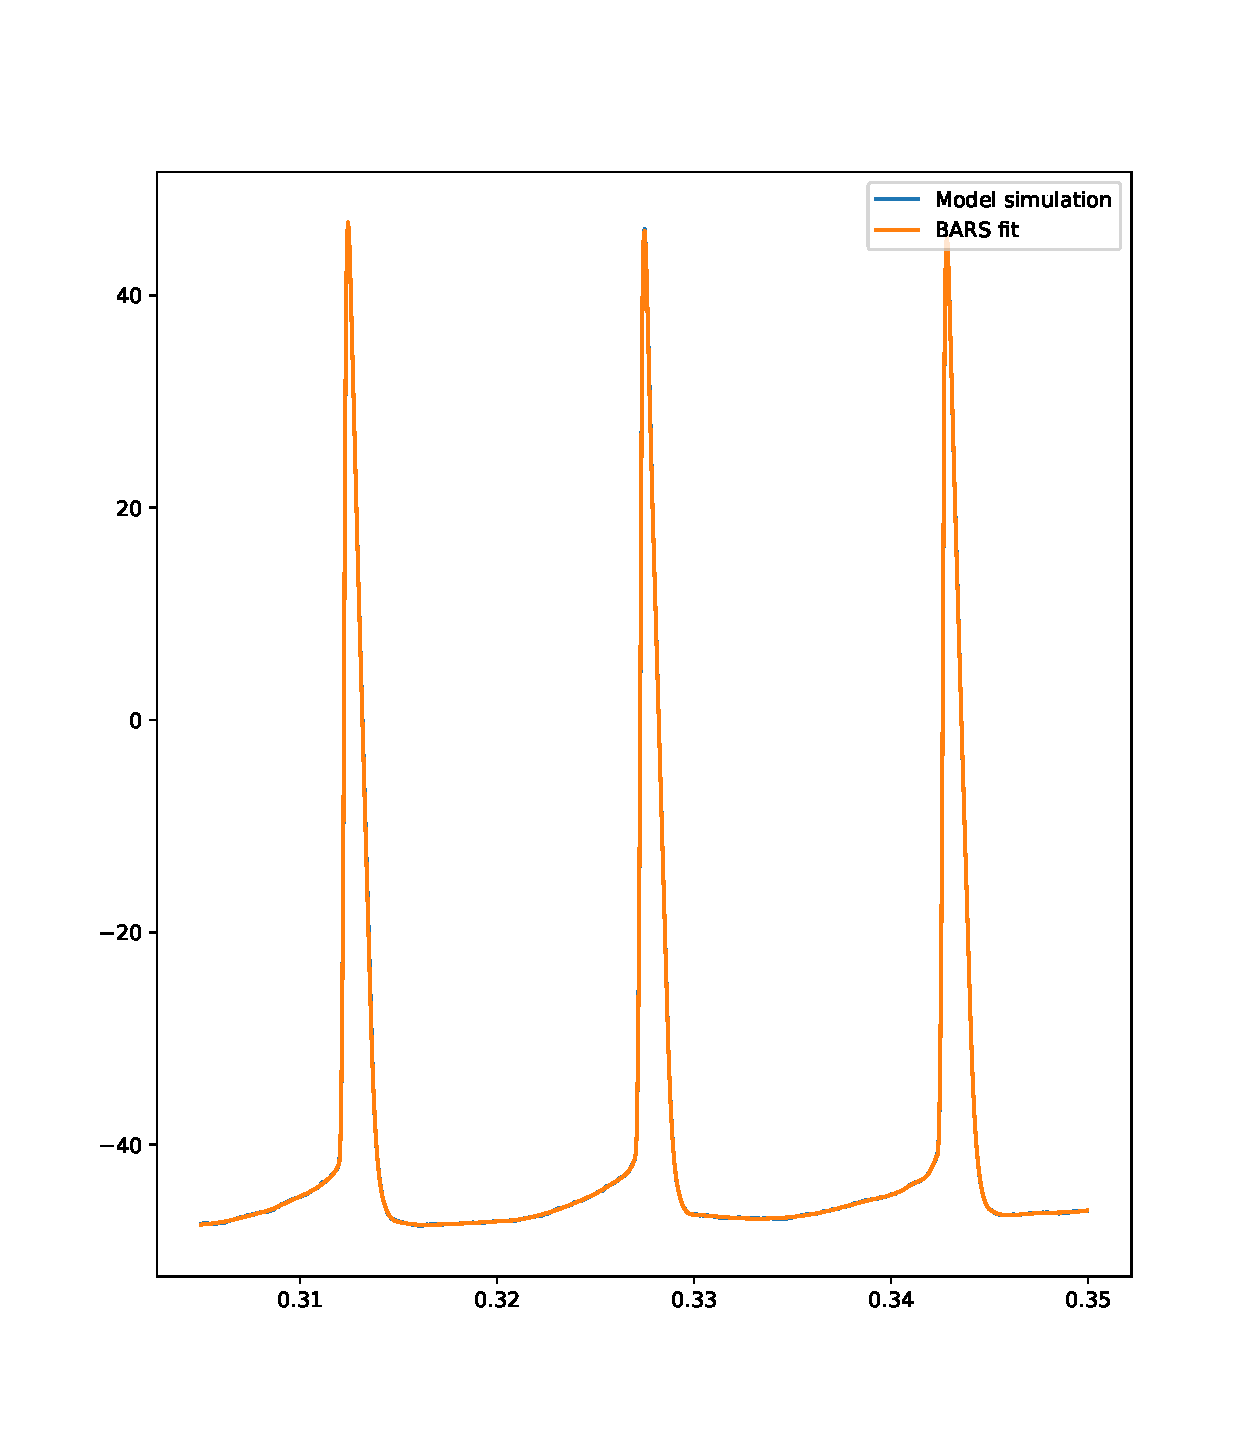
\includegraphics[width=1.1\textwidth]{./BARS.pdf}
\end{center}
\end{column}



\begin{column}{0.5\columnwidth}
\begin{center}
GPR (SEKernel)
\end{center}

\begin{center}
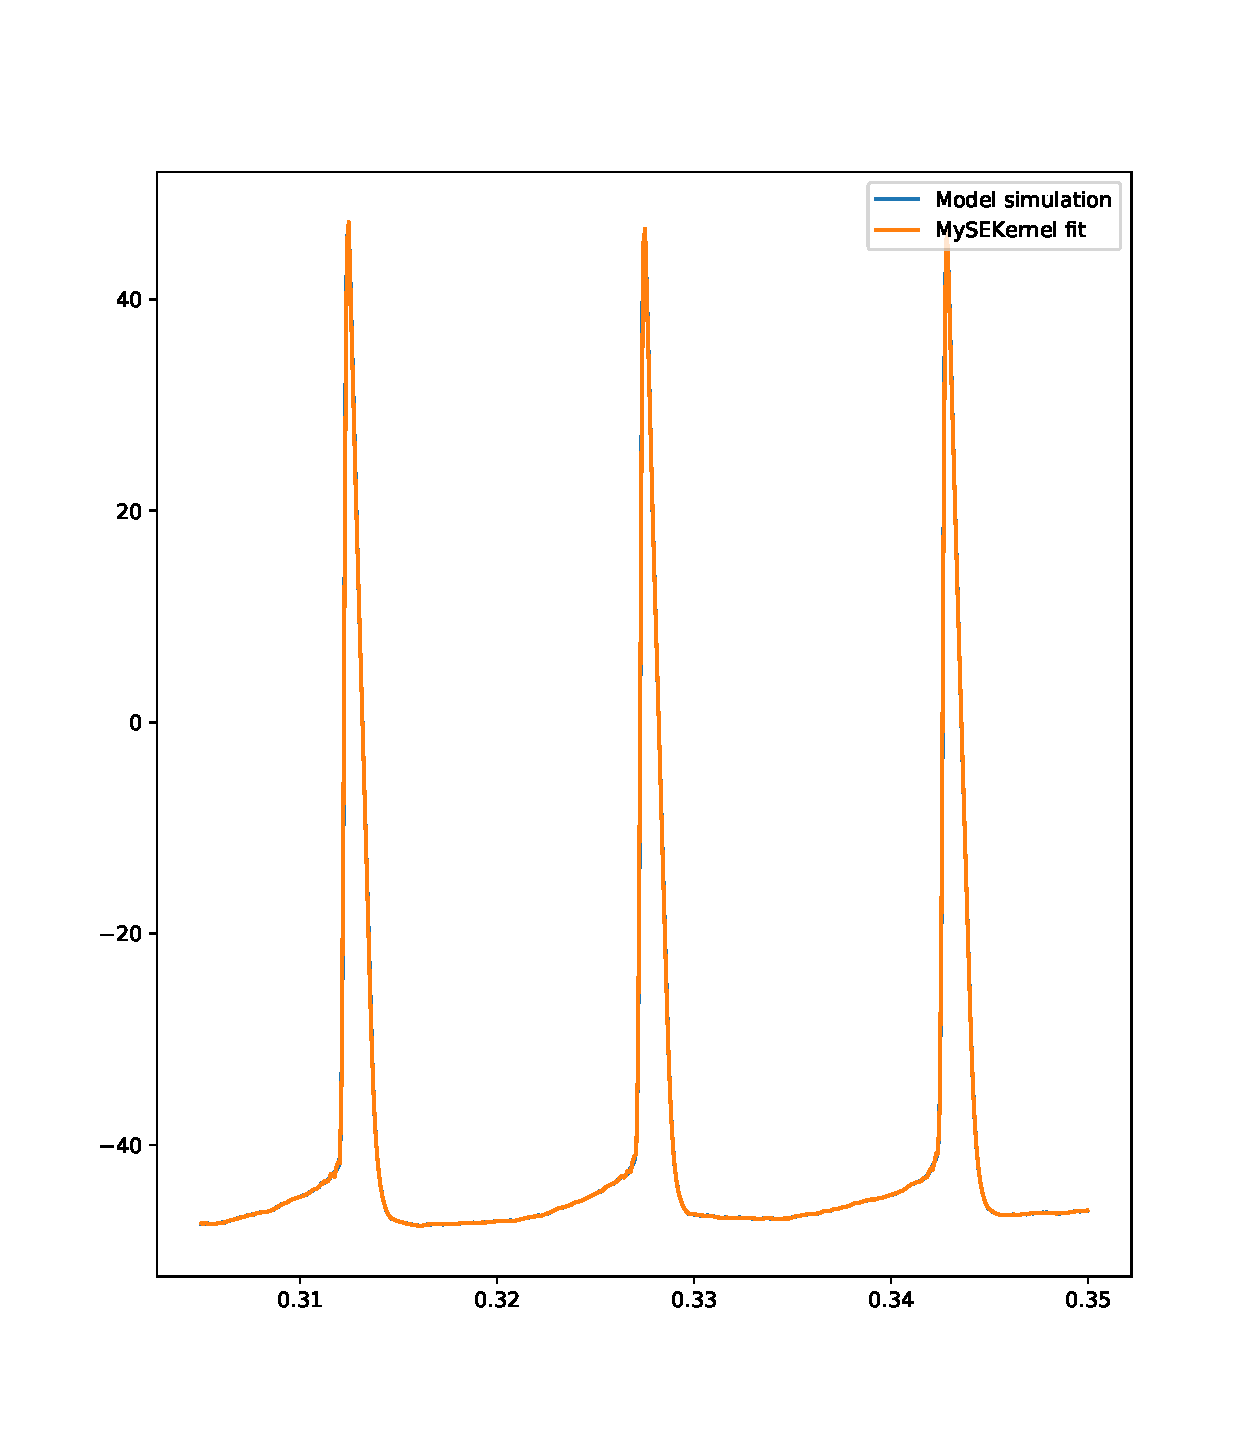
\includegraphics[width=1.1\textwidth]{./SEKernel_f_6d23e2_l_5d71e-8_n_0d1.pdf}
\end{center}
\end{column}
\end{columns}
\end{frame}


\begin{frame}[plain,label={sec:org8dbeab2}]{Splines vs GPR}
\begin{columns}
\begin{column}{0.5\columnwidth}
\begin{center}
Splines
\end{center}

\begin{center}
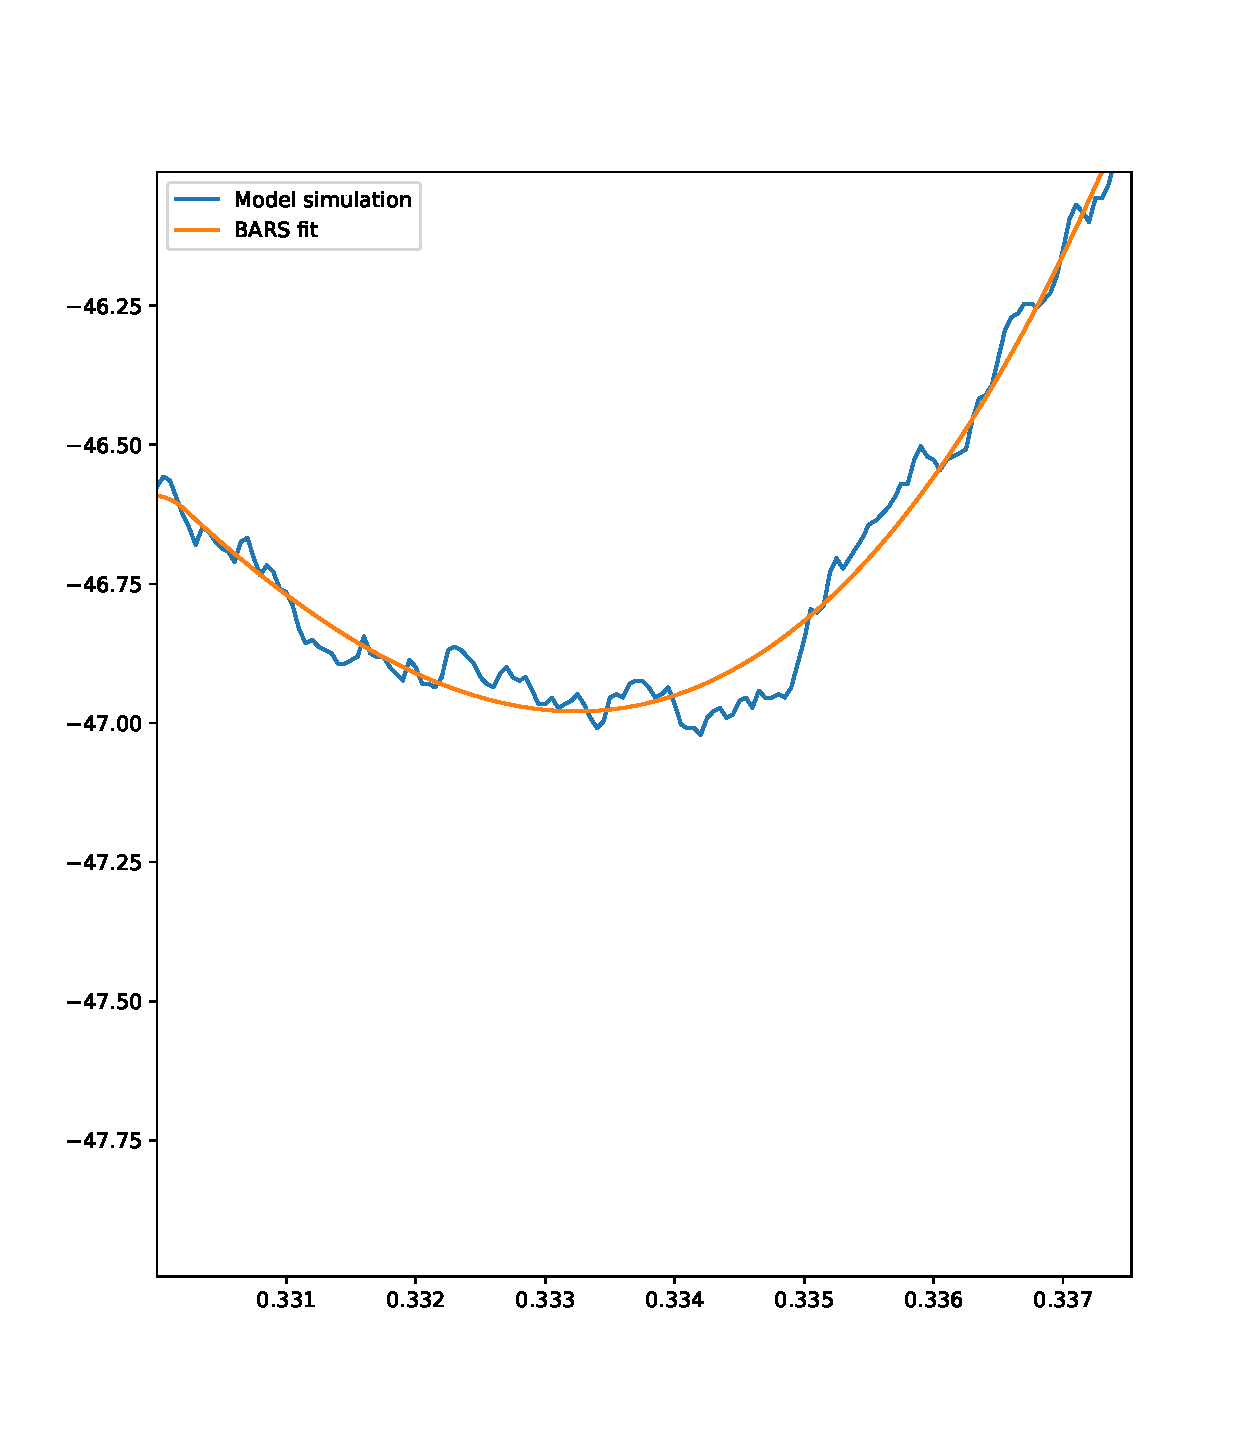
\includegraphics[width=1.1\textwidth]{./BARS2.pdf}
\end{center}    
\end{column}


\begin{column}{0.5\columnwidth}
\begin{center}
GPR (SEKernel)
\end{center}

\begin{center}
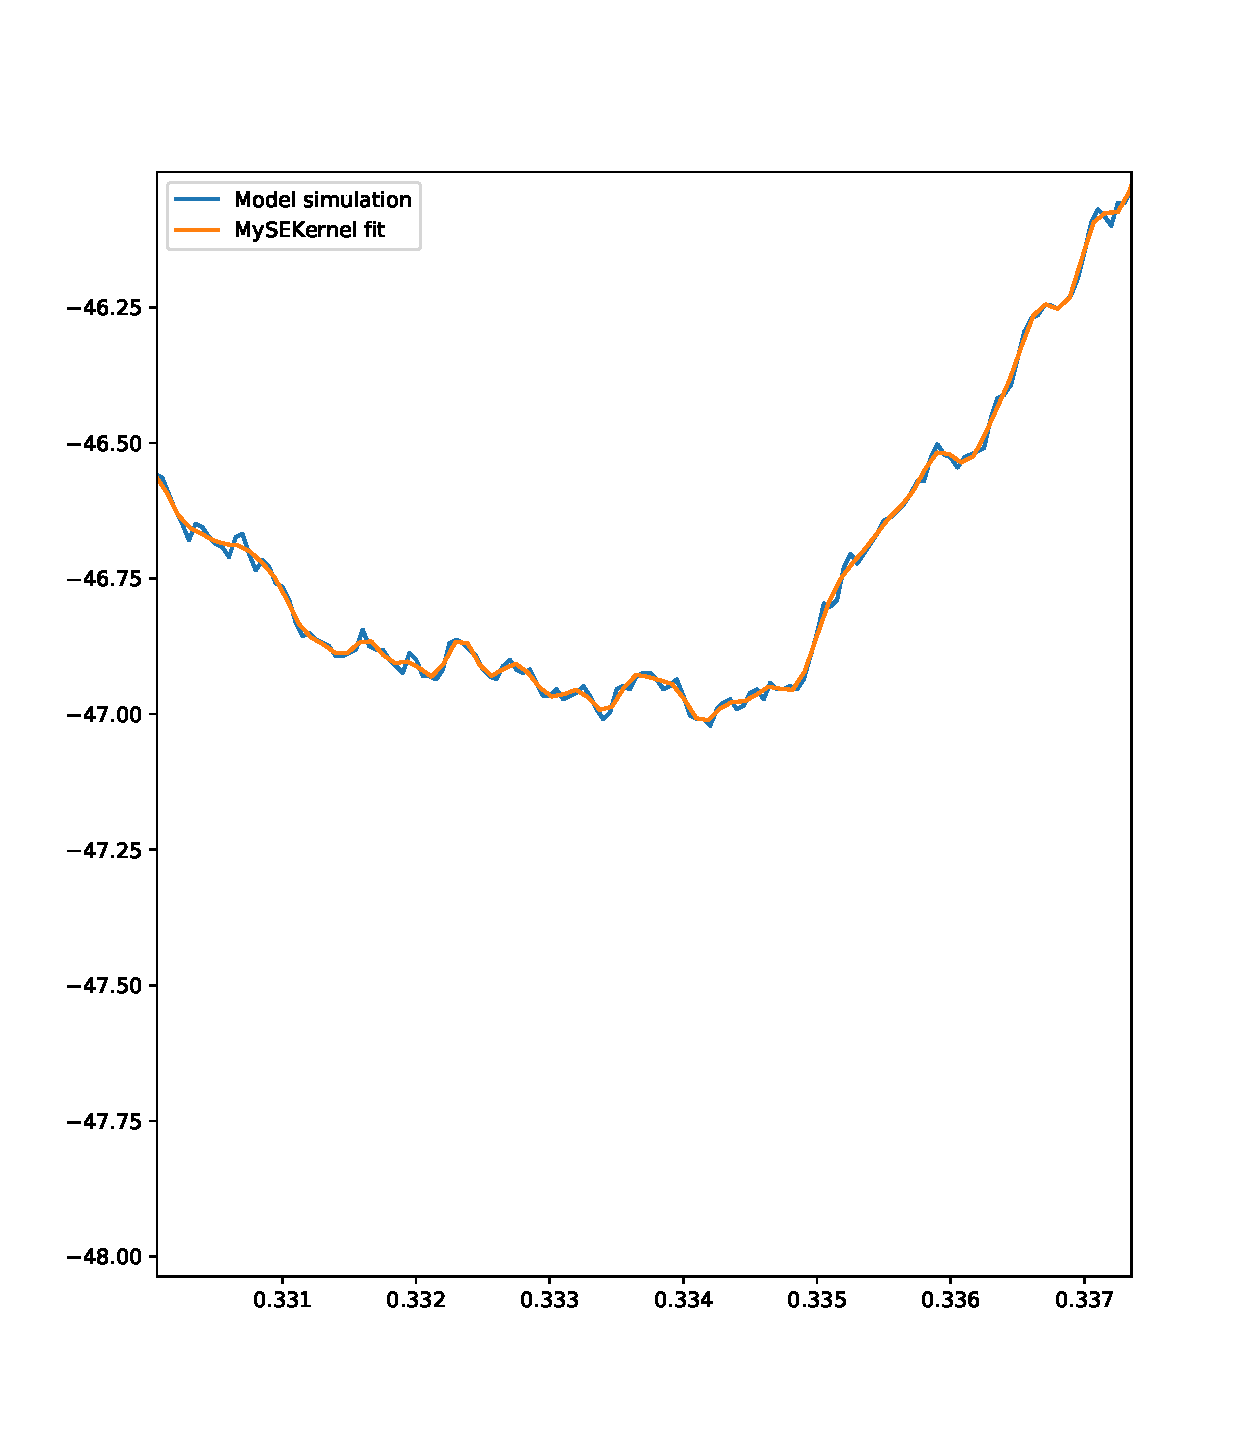
\includegraphics[width=1.1\textwidth]{./SEKernel2.pdf}
\end{center}
\end{column}
\end{columns}
\end{frame}


\begin{frame}[label={sec:org4b5a1fa}]{Real data, splines model}
\begin{center}
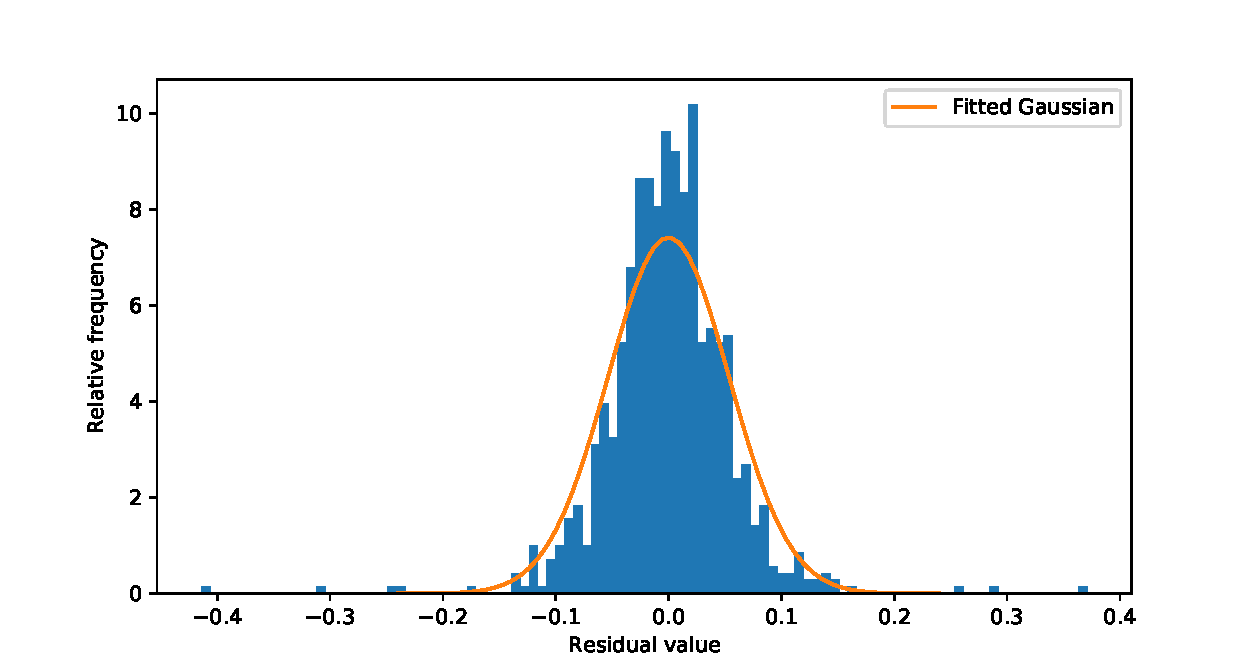
\includegraphics[width=.9\textwidth]{./hist.pdf}
\end{center}
\vfill
\end{frame}


\begin{frame}[plain,label={sec:org38c56f4}]{Not perfect, but good enough}
\begin{columns}
\begin{column}{0.5\columnwidth}
\begin{center}
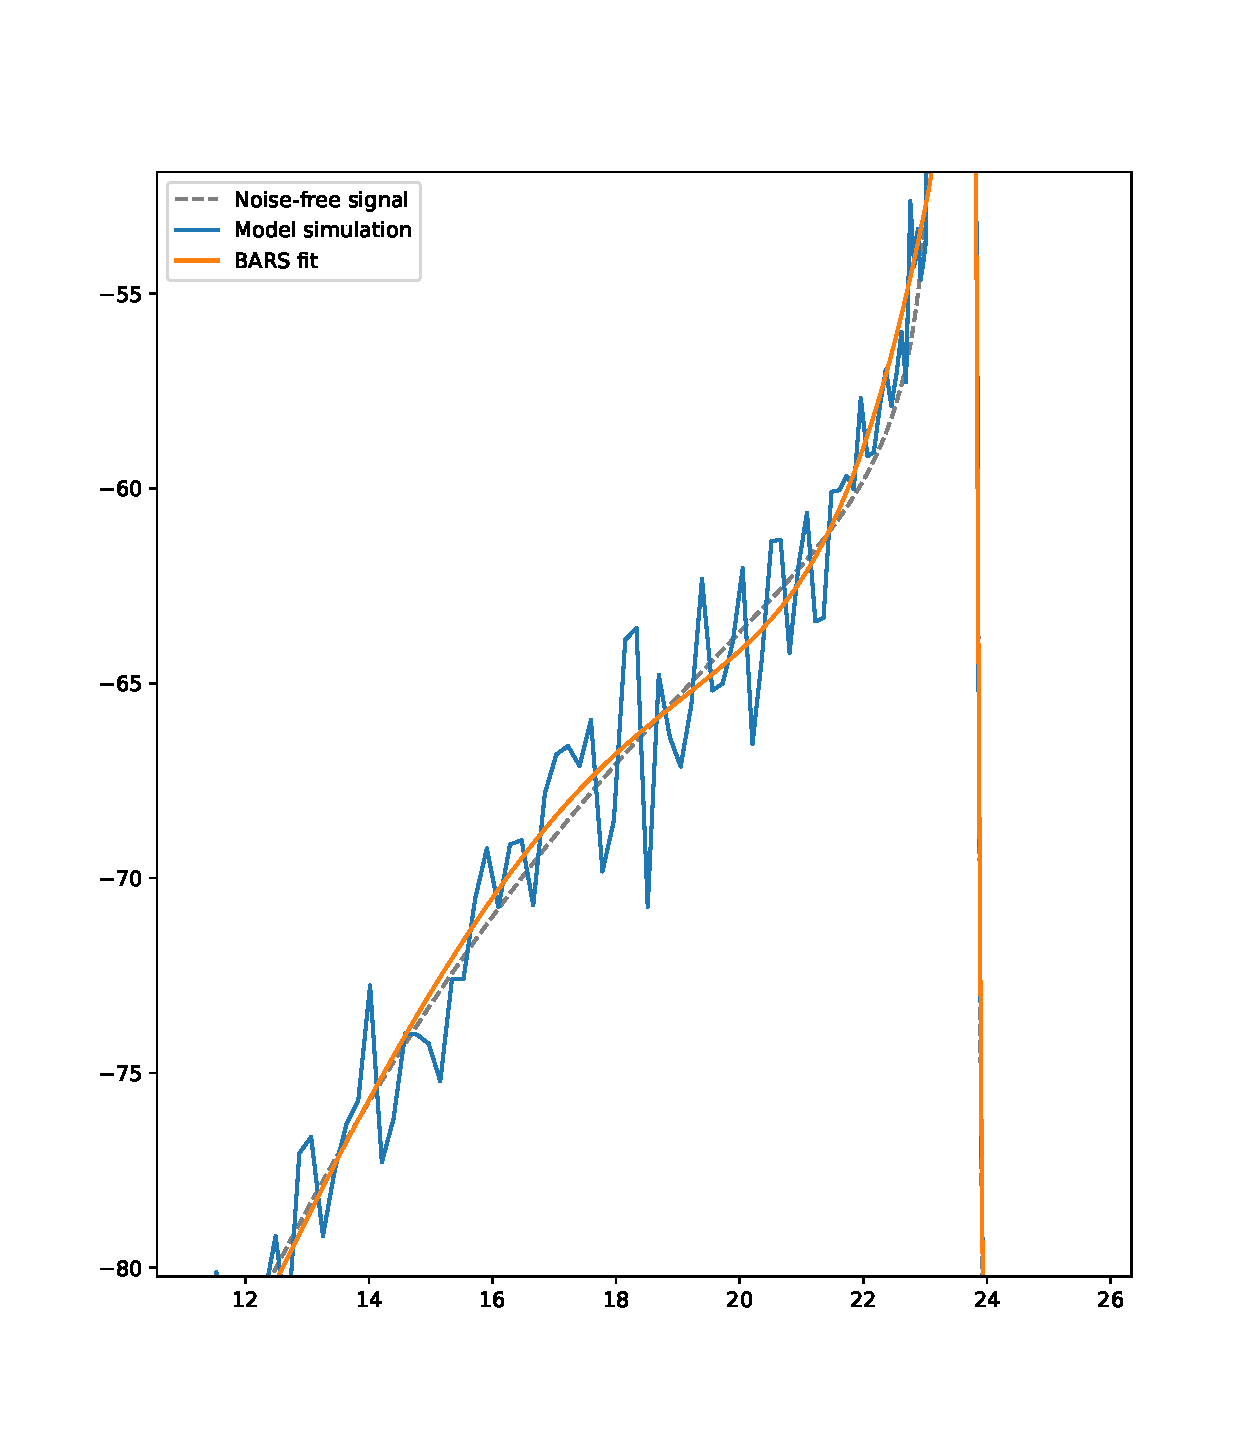
\includegraphics[width=1.1\textwidth]{./barsbad3.pdf}
\end{center}
\end{column}

\begin{column}{0.5\columnwidth}
\begin{center}
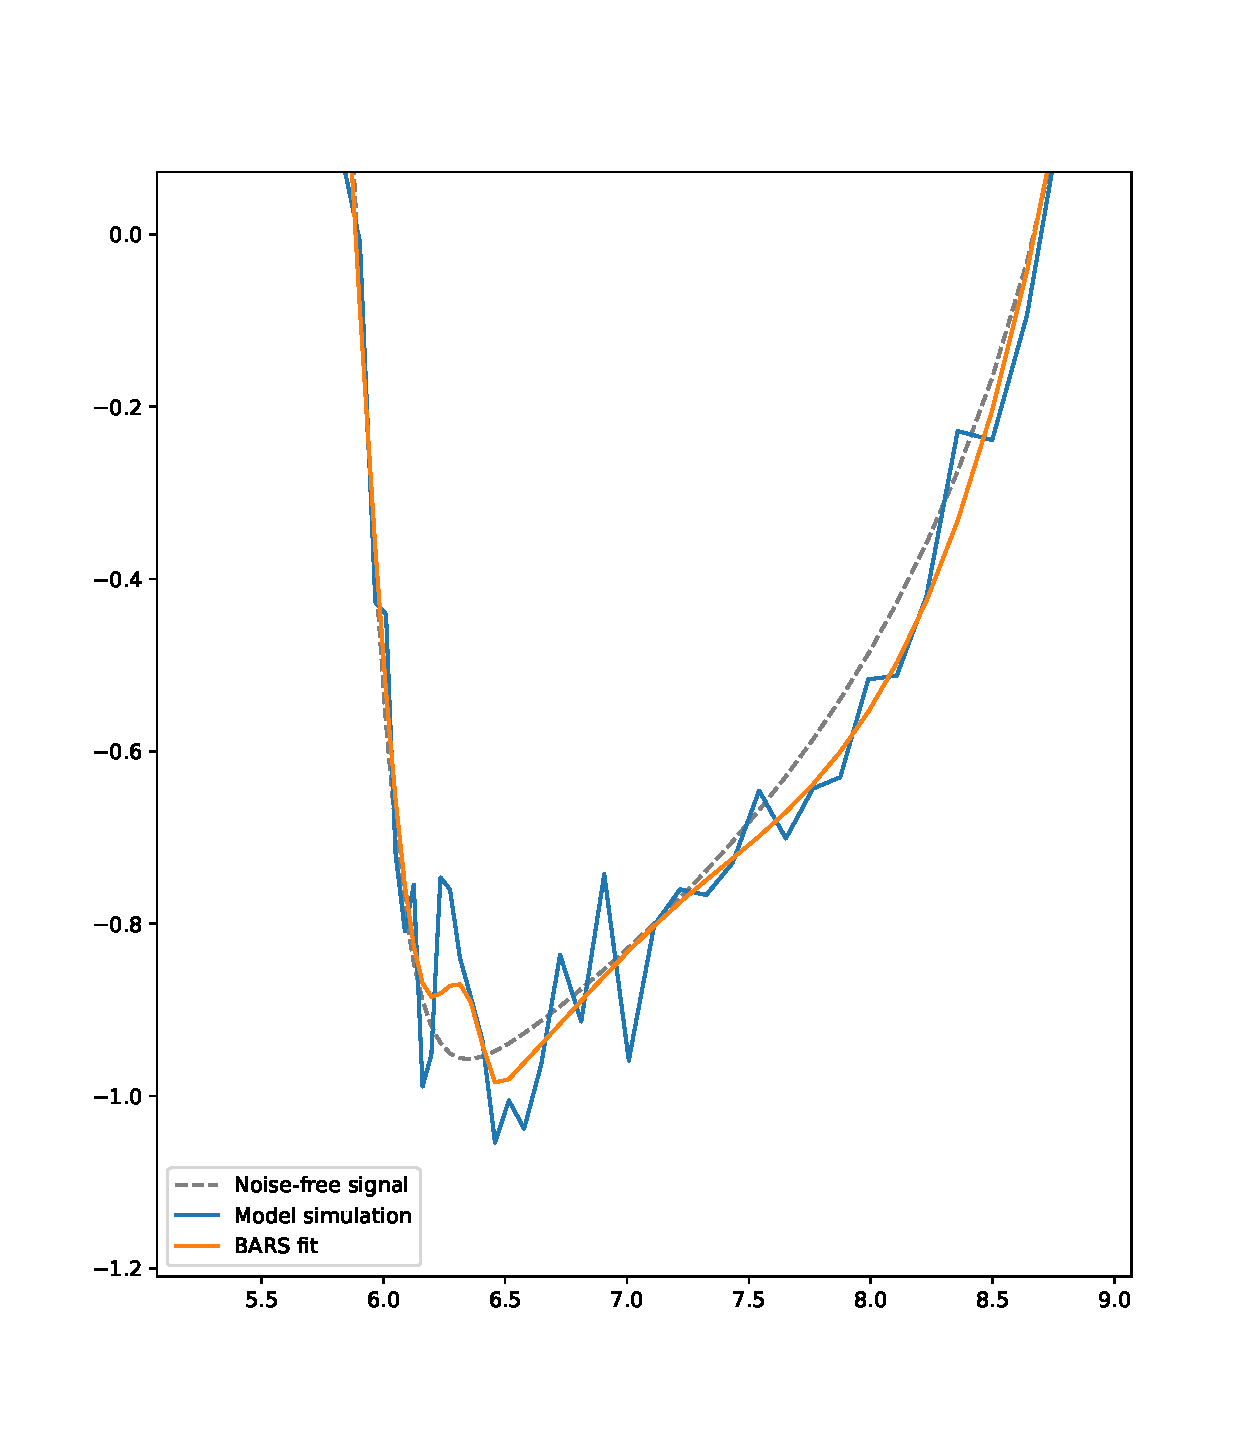
\includegraphics[width=1.1\textwidth]{./barsbad2.pdf}
\end{center}
\end{column}
\end{columns}
\end{frame}


\begin{frame}[label={sec:org0a0d345}]{Splines caveats}
\begin{itemize}[<+->]
\item BARS works well, without any hyperparameter tuning
\item ISSUE: I don't know how or why it works
\begin{itemize}
\item Can't rigorously justify why it's a good method
\item Can't predict when it would work and when it would fail
\item Can't determine good hyperparameter values
\end{itemize}
\item ISSUE: haven't implemented it
\begin{itemize}
\item Relying on some old \emph{C} code to make it run
\item \emph{C} implementation evaluates the splines model at the training points, and returns them
\item Can't evaluate model at non-training points; doesn't give a continuous (interpolating) model, \emph{can't be validated!}
\end{itemize}
\item ISSUE: harder to encode periodicity
\begin{itemize}
\item Periodic kernels almost surely (probability 1) give periodic posteriors
\item Periodic splines are a thing, maybe try periodic BARS?
\end{itemize}
\end{itemize}
\end{frame}


\section{Other ideas}
\label{sec:org30d9468}
\begin{frame}[label={sec:org9ab271b}]{Abandoned ideas}
\begin{itemize}
\item Generalised spectral mixture kernels
\begin{itemize}
\item Couldn't get them to train
\end{itemize}
\end{itemize}

\vfill
\begin{itemize}
\item Support vector regression
\begin{itemize}
\item Couldn't find any justification to use this over GPR
\end{itemize}
\end{itemize}

\vfill
\begin{itemize}
\item Latent ODEs / neural ODEs / physics-informed NNs
\begin{itemize}
\item Would require state-space reconstruction, doesn't seem like a beneficial use of time
\end{itemize}
\end{itemize}
\end{frame}


\begin{frame}[label={sec:org621f6a2}]{Other models for a paper}
\begin{itemize}
\item NARMAX
\item Wavelets
\item Warping GPs
\begin{itemize}
\item Either learn a warp\ldots{}
\item \ldots{}or apply a simple transformation to the data (log, exp, logistic, \ldots{})
\end{itemize}
\item Deep GPs
\item Hybrid methods
\item Other nonparametric methods
\begin{itemize}
\item RKHS, KNN, etc.
\end{itemize}
\end{itemize}
\end{frame}


\section{Next steps}
\label{sec:orgb73c317}
\begin{frame}[label={sec:orge295d5c}]{Next steps}
\begin{itemize}[<+->]
\item Dig into free-knot splines literature
\begin{itemize}
\item BARS and other free-knot methods
\end{itemize}
\item Understand how and why it works
\begin{itemize}
\item Useful for justifying why it's a good model, and when it will and won't work
\item Will help decide whether periodic BARS is possible
\end{itemize}
\item Write up my own implementation
\begin{itemize}
\item Allows for validation, interpolation
\end{itemize}
\end{itemize}

Then\ldots{}
\begin{itemize}[<+->]
\item Other data sources
\item Warping GPs, deep GPs, NARMAX, etc.
\item MATLAB wrapper?
\begin{itemize}
\item Having ready-to-go codes might make a paper more popular
\end{itemize}
\end{itemize}
\end{frame}


\section{GPR tests}
\label{sec:orgf7b5f33}

\begin{verbatim}
./model_tester.py -d HRFast -m MySEKernel

./model_tester.py -d HindmarshRose -m Matern32 -p CleanFitted 
		  -r 1e-6 -V

./model_tester.py -d FitzhughNagumo -m ModuloKernel -r 1e-6 
		  -n 0.1

./model_tester.py -d HodgkinHuxley -m PeriodicKernel -o

./model_tester.py -d 08o28004_channel_0_sweep_8.np -m 
		  MySEKernel -f 6.23e2 -l 5.71e-8 -n 0.1
\end{verbatim}
\end{document}
